% !TEX TS-program = pdflatex
% !TEX encoding = UTF-8 Unicode

% Setting up the document class for a character sheet
\documentclass[10pt, a4paper]{article}

% Including essential packages for encoding and font setup
\usepackage[utf8]{inputenc}
\usepackage[T1]{fontenc}
\usepackage{helvet}
\usepackage{amssymb}
\usepackage{graphicx}
\renewcommand{\familydefault}{\sfdefault}

% Configuring page geometry for a landscape layout
\usepackage{geometry}
\geometry{a4paper, landscape, margin=1cm, top=1cm, bottom=1.5cm}

% Defining colors for box styling
\usepackage{xcolor}
\definecolor{boxheaderbg}{HTML}{000000}
\definecolor{boxheaderfg}{HTML}{FFFFFF}
\definecolor{boxcontentbg}{HTML}{F0F0F0}
\definecolor{boxborder}{HTML}{000000}

% Setting up tcolorbox for styled, fixed-size boxes
\usepackage[many]{tcolorbox}

% Adding hyperref for interactive form fields
\usepackage{hyperref}

% Configuring headers and footers
\usepackage{fancyhdr}
\pagestyle{fancy}
\fancyhf{}
\fancyfoot[R]{\footnotesize "Fail Forward character sheet" by Visa Lampi is licensed under CC BY-NC 4.0.}
\renewcommand{\headrulewidth}{0pt}
\renewcommand{\footrulewidth}{0pt}

% Including tabularx for potential table formatting
\usepackage{tabularx}

\begin{document}

% Starting the form environment for interactive fields
\begin{Form}

% Creating a two-column layout using minipages
\begin{minipage}[t]{0.48\textwidth}
    \vspace{0pt}
    % Defining the CHARACTER box with a placeholder image and name field
    \begin{tcolorbox}[
        width=12.5cm,
        height=4.5cm,
        title=CHARACTER,
        colback=boxcontentbg,
        colframe=boxborder,
        coltitle=boxheaderfg,
        colbacktitle=boxheaderbg,
        fonttitle=\bfseries\sffamily\small,
        clip upper,
        before skip=0pt
    ]
        \begin{minipage}[t][4cm]{0.22\linewidth}
            \centering
            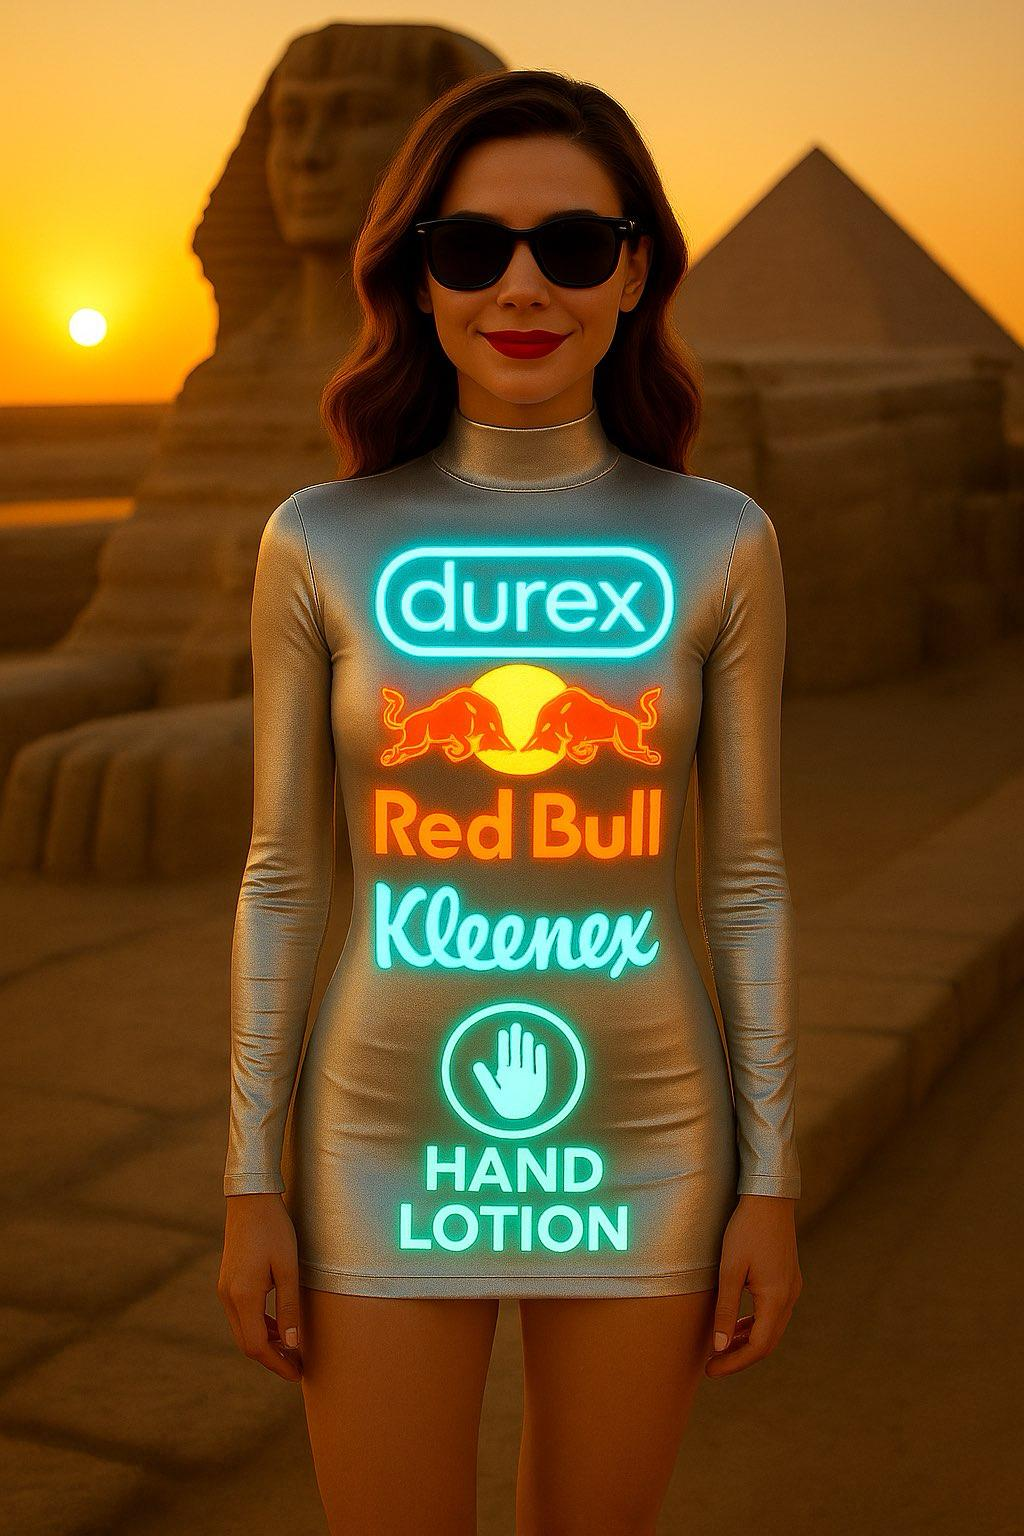
\includegraphics[width=0.9\linewidth, height=3.8cm, keepaspectratio=true]{Nova.jpg}
            \vspace{0pt}
        \end{minipage}%
        \hspace{0.2cm}%
        \begin{minipage}[t][4cm]{0.74\linewidth}
            \centering
            \TextField[name=character_name, width=8cm, height=2cm, multiline=true, default={Nova Cleo @CleoOnlyFans}, charsize=20pt, backgroundcolor=boxcontentbg, borderwidth=0, bordercolor=boxcontentbg]{}
        \end{minipage}
    \end{tcolorbox}

    \vspace{3mm}

    % Defining the BACKGROUND box with Nova Cleo's bio
    \begin{tcolorbox}[
        width=12.5cm,
        height=6.5cm,
        title=BACKGROUND,
        colback=boxcontentbg,
        colframe=boxborder,
        coltitle=boxheaderfg,
        colbacktitle=boxheaderbg,
        fonttitle=\bfseries\sffamily\small,
        clip upper,
        before skip=0pt
    ]
        \TextField[name=background, width=11.5cm, height=5.5cm, multiline=true, default={Nova Cleo (@CleoOnlyFans) isn't your average content creator---she's an icon in silver, turning the Egyptian sands into her personal runway. With 3.5M subscribers on OnlyFans, she's become a sensation in the tech-fashion crossover space. Blending Cleopatra vibes with sci-fi chic, she's here to dominate timelines and hearts. A rising star for nerd boys who love brains with their beauty, she crafts every shot like a story. Her content? Part cosplay, part queen, all captivating. Her unique blend of ancient aesthetics and modern tech has made her a sought-after brand ambassador for cutting-edge technology companies.}, backgroundcolor=boxcontentbg, borderwidth=0, bordercolor=boxcontentbg]{}
    \end{tcolorbox}

    \vspace{3mm}

    % Defining the ABILITIES box with 6 options (choose 3)
    \begin{tcolorbox}[
        width=12.5cm,
        height=4cm,
        title=ABILITIES (choose 3),
        colback=boxcontentbg,
        colframe=boxborder,
        coltitle=boxheaderfg,
        colbacktitle=boxheaderbg,
        fonttitle=\bfseries\sffamily\small,
        clip upper,
        before skip=0pt
    ]
        \TextField[name=abilities, width=11.5cm, height=3cm, multiline=true, default={\newlinechar Social Media Domination \qquad \hspace{10mm} Cosplay Creativity \newline \qquad \newline Sci-Fi Aesthetic \qquad \hspace{10mm} Captivating Storytelling \newline \qquad \newline Viral Marketing \qquad \hspace{10mm} Cultural Fusion Yoga & Meditation}, backgroundcolor=boxcontentbg, borderwidth=0, bordercolor=boxcontentbg]{}
    \end{tcolorbox}
\end{minipage}
\hfill
\begin{minipage}[t]{0.48\textwidth}
    \vspace{0pt}
    % Defining the SANITY box (unchanged)
    \begin{tcolorbox}[
        width=12.5cm,
        height=2.5cm,
        title=SANITY,
        colback=boxcontentbg,
        colframe=boxborder,
        coltitle=boxheaderfg,
        colbacktitle=boxheaderbg,
        fonttitle=\bfseries\sffamily\small,
        clip upper,
        before skip=0pt
    ]
        \begin{minipage}[t]{\linewidth}
            \large \hspace*{2mm}
            $\bigcirc$ \hspace{1em}
            $\bigcirc$ \hspace{1em}
            $\bigcirc$ \hspace{1em}
            $\bigcirc$ \hspace{1em}
            $\bigcirc$ \hspace{1em}
            $\bigcirc$ \\
            \textit{\footnotesize \hspace*{2mm} (6 = Sanity breaks)} \\
            \vspace{2mm}
            \textit{\footnotesize \hspace*{2mm} Check one circle each time sanity decreases.}
        \end{minipage}
    \end{tcolorbox}

    \vspace{3mm}

    % Defining the PERSONALITY box with 4 options (choose 2)
    \begin{tcolorbox}[
        width=12.5cm,
        height=3.5cm,
        title=PERSONALITY (choose 2),
        colback=boxcontentbg,
        colframe=boxborder,
        coltitle=boxheaderfg,
        colbacktitle=boxheaderbg,
        fonttitle=\bfseries\sffamily\small,
        clip upper,
        before skip=0pt
    ]
        \TextField[name=personality, width=11.5cm, height=2.5cm, multiline=true, default={Charismatic  Bold  Creative  Eccentric}, backgroundcolor=boxcontentbg, borderwidth=0, bordercolor=boxcontentbg]{}
    \end{tcolorbox}

    \vspace{3mm}

    % Defining the HANDICAPS box with 4 options (choose 2)
    \begin{tcolorbox}[
        width=12.5cm,
        height=3.5cm,
        title=HANDICAPS (choose 2),
        colback=boxcontentbg,
        colframe=boxborder,
        coltitle=boxheaderfg,
        colbacktitle=boxheaderbg,
        fonttitle=\bfseries\sffamily\small,
        clip upper,
        before skip=0pt
    ]
        \TextField[name=handicaps, width=11.5cm, height=2.5cm, multiline=true, default={Attention-Seeking  Cultural Misunderstanding  Overconfidence  Tech-Dependency}, backgroundcolor=boxcontentbg, borderwidth=0, bordercolor=boxcontentbg]{}
    \end{tcolorbox}

    \vspace{3mm}

    % Defining the EQUIPMENT box with 8 options (choose 4)
    \begin{tcolorbox}[
        width=12.5cm,
        height=5cm,
        title=EQUIPMENT (choose 4),
        colback=boxcontentbg,
        colframe=boxborder,
        coltitle=boxheaderfg,
        colbacktitle=boxheaderbg,
        fonttitle=\bfseries\sffamily\small,
        clip upper,
        before skip=0pt
    ]
        \TextField[name=equipment, width=11.5cm, height=4cm, multiline=true, default={Smartphone  LED Bodysuit  Portable Ring Light  Designer Sunglasses  Tripod  Neon Accessories  Camera Drone  Makeup Kit  Mushrooms  Smoke Grenades  Derringer}, backgroundcolor=boxcontentbg, borderwidth=0, bordercolor=boxcontentbg]{}
    \end{tcolorbox}
\end{minipage}

% Ending the form environment
\end{Form}

\end{document}